\documentclass{article}

% Language setting
% Replace `english' with e.g. `spanish' to change the document language
\usepackage[english]{babel}

% Set page size and margins
% Replace `letterpaper' with `a4paper' for UK/EU standard size
\usepackage[letterpaper,top=2cm,bottom=2cm,left=3cm,right=3cm,marginparwidth=1.75cm]{geometry}

% Useful packages
\usepackage{amsmath}
\usepackage{amssymb}
\usepackage{graphicx}
\usepackage[colorlinks=true, allcolors=blue]{hyperref}

\begin{document}

\section{The Standard Model}

\subsection{History of the Standard Model}

The building blocks of our prevailing picture of elementary particle physics were established over the course of decades by experimental discoveries and theoretical advances, culminating in the development of a theoretical framework known as the Standard Model (SM). In the 1880s, the electron was the first subatomic particle to be identified, through measurements of particles produced by ionizing gas. By the 1930s, atoms were known to consist mostly of empty space, with protons and neutrons concentrated at the center and orbited by electrons. Spurred by advances in particle accelerator technology, the experimental discoveries of the positron, the muon, and the pion, painted an increasingly complicated picture of particle physics that could not be described solely with atomic physics.

In the absence of a theoretical framework describing these particles, in the 1960s and 1970s physicists and mathematicians developed the Standard Model to describe and encompass these fundamental particles and the forces that govern their interactions. The particle content of the Standard Model is shown in Fig. \ref{fig:intro-standard-model}: they are grouped into fermions, which comprise all known matter, and bosons, which mediate the interactions between particles.

Fermions consist of quarks and leptons, and are grouped into three generations. For example, the electron belongs to the first generation of leptons. The second and third generation counterparts of the electron are the muon and the tau lepton, and are over 200 and 30,000 times heavier than the electron respectively. Bosons are force carriers; the interaction of fermions with bosons corresponds to fundamental forces. The Standard Model describes the electromagnetic force, the strong nuclear force, and the weak nuclear force.

% https://en.wikipedia.org/wiki/File:Standard_Model_of_Elementary_Particles.svg
\begin{figure}[ht]
    \centering
    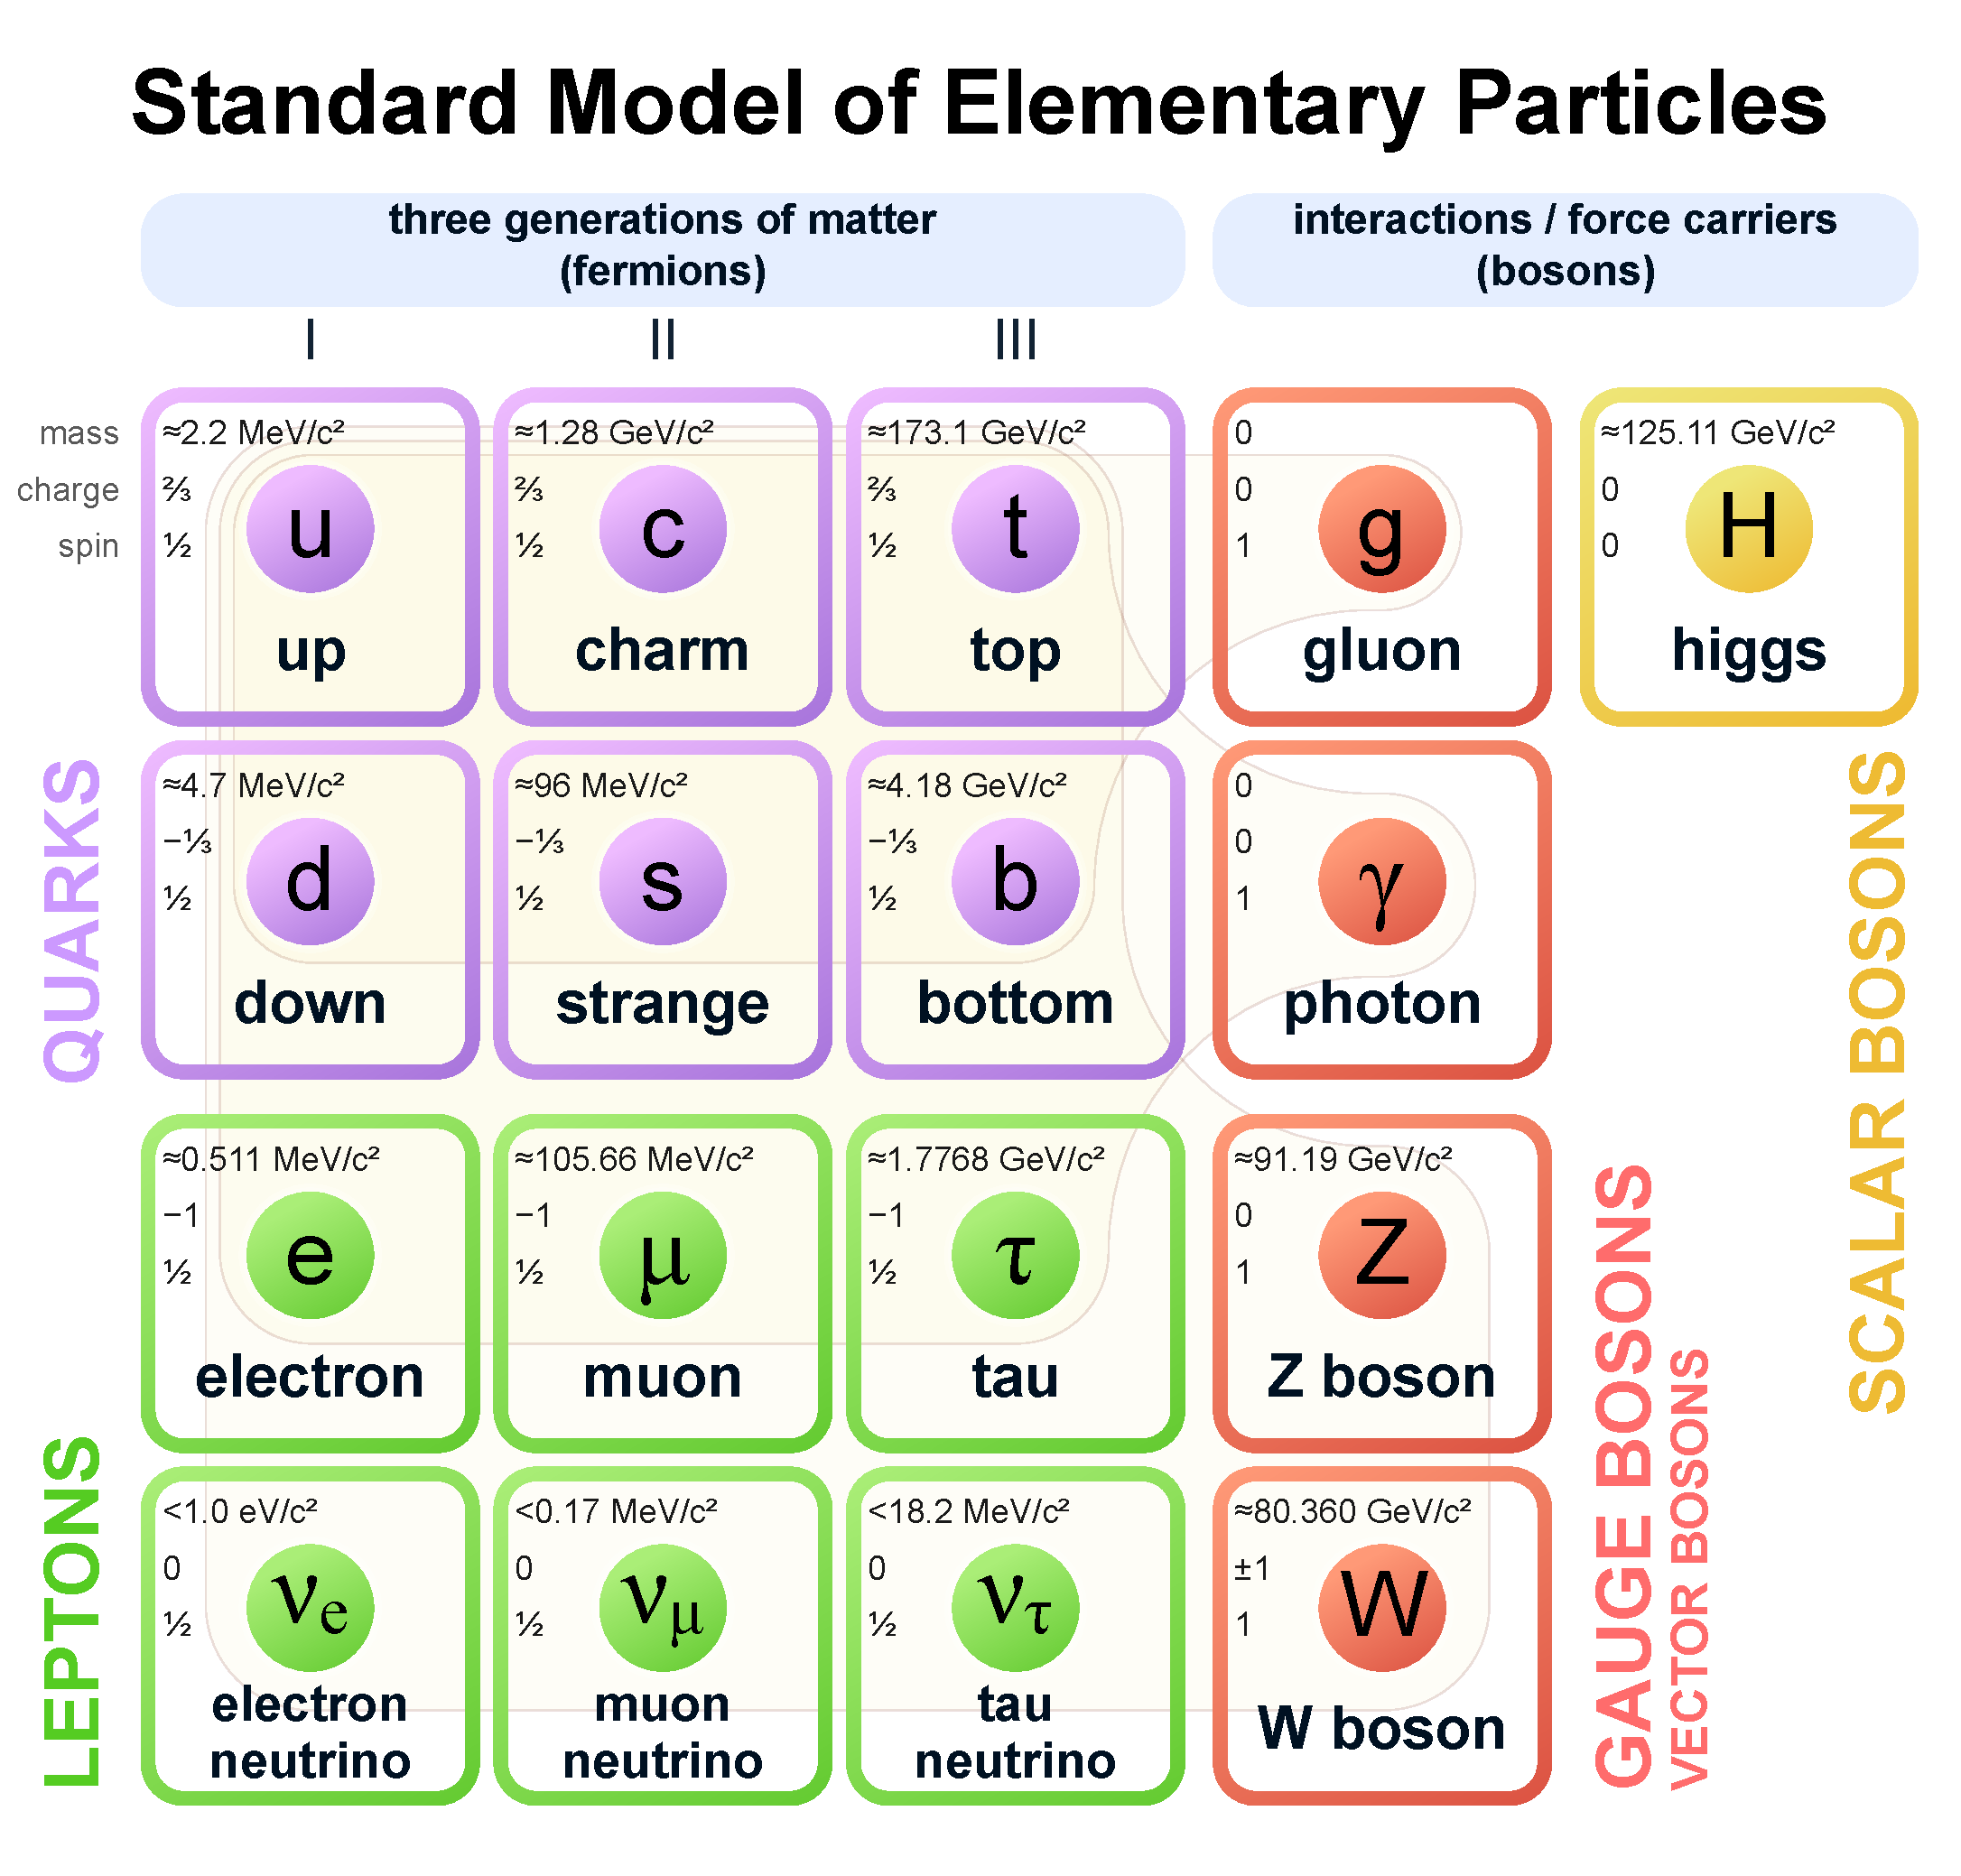
\includegraphics[width=8cm]{figures/Standard_Model_of_Elementary_Particles.pdf}
    \caption{Table of Standard Model particles [CITE], showing the grouping of the fermions into three generations of matter and the bosons, responsible for carrying the three fundamental forces in the Standard Model. The masses, charges, and spins of the particles are shown. The antimatter counterparts of the fermions are not shown. The possible interactions between the fermions and gauge bosons are highlighted.}
    \label{fig:intro-standard-model}
\end{figure}





\subsection{The Standard Model as a gauge theory}

\subsubsection{Gauge invariance}

In this section we turn to a mathematical description of the structure of the Standard Model, specifically from the angle of gauge theories,

An example from classical physics is the electromagnetic interaction, where the fundamental field is the four-vector potential $A^\mu$. The physical electromagnetic fields and Maxwell's equations arise from the elements of the tensor $F_{\mu\nu}(x) = \partial_\mu A_\nu (x) - \partial_\nu A_\mu (x)$. Any two choices of $A^\mu$ that are related by a transformation of the form \begin{equation} A_\mu \rightarrow A_\mu + \partial_\mu \alpha \label{eqn:gauge_symmetry}\end{equation} for any real, differentiable function $\alpha(x)$, describe the same physical configuration, and has no effect on Maxwell's equations. This transformation in Eqn. \ref{eqn:gauge_symmetry} is often referred to as a \textbf{gauge symmetry}, but can also be thought of as \textbf{gauge redundancy}.


In gauge theories, the freedom of choice of gauge states that the existence and form of an interaction can be deduced from the existence of physically indeterminate, gaugable quantities.

Noether's theorem states that for every global transformation under which the Lagrangian density is invariant, there exists a conserved quantity. If $\mathcal{L}(\Psi(x), \partial_\mu \Psi(x))$ is invariant under the transformation of the wave function $\Psi(x) \rightarrow \Psi'(x)$, where $\Psi'(x) = \Psi(x) + \delta \Psi(x)$, then there exists a conserved current 
\begin{equation}
    \partial_\mu \left( \frac{\partial\mathcal{L}(x)}{\partial(\partial_\mu \Psi(x))} \delta \Psi(x)  \right) = 0
\end{equation}


\subsubsection{Local gauge symmetries}
If we modify the wave function with a phase transformation $\Psi'(x) = \exp(i e \chi) \Psi(x)$, and we allow the phase $\chi$ to be a function of spacetime, we introduce \textbf{interactions} to the theory. A wave function of the form
\begin{equation}
    \Psi'(x) = \exp(i e \chi(x)) \Psi(x)
\end{equation}
can be verified, to be not a solution to the Dirac equation for free particles: $(i \gamma^\mu \partial_\mu - m) \Psi(x) = 0$. To take the derivative of a vector field $V(x)$ (e.g. a Dirac wave function), at two displaced space-time points, in a curvilinear coordinate system, 
\begin{equation}
    \mathcal{D}_\mu \equiv \lim_{\Delta x^\mu \rightarrow 0} \frac{V_{\parallel}(x + \Delta x) - V(x)}
{\Delta x^\mu}\end{equation}

To write a derivative that is covariant under this transformation, we define a \textbf{covariant derivative}, where $A_\mu(x)$ is a 4-vector potential:
\begin{equation}
    D_\mu = \partial_\mu + i e A_\mu
\label{eqn:modified_dirac}
\end{equation}
which gives the modified Dirac equation:
\begin{equation}
    \left( i \gamma^\mu \mathcal{D}_\mu - m  \right) \Psi(x) = 0
\end{equation}
The simultaneous gauge transformation $A'_\mu(x) = A_\mu(x) - \partial_\mu\chi(x)$ and wavefunction transformation $\Psi'(x) = \exp(ie\chi(x)) \Psi(x)$ leaves the covariant-derivative form of the Dirac equation (Eqn \ref{eqn:gauge_symmetry}) invariant.

To generalize this, if the theory is invariant for unitary transformations $U$ of the particle states according to 
\begin{equation}
    \Psi' = U\Psi
\label{eqn:generic_unitary_transformation}
\end{equation}
We want to define a derivative
\begin{equation}
    D^\mu = \partial^\mu + ig B^\mu
\end{equation}
that keeps the theory invariant under Eqn. \ref{eqn:generic_unitary_transformation}. The four-potential $B^\mu$ represents the interacting four-potential which must be added to keep the theory invariant.

The Standard Model is built around the gauge transformations $G = SU(3) \times SU(2) \times U(1)$. $SU(3)$ is associated to the strong force; $SU(2)$ is associated to the weak force; and $U(1)$ is hypercharge. Electromagnetism arises from the terms $SU(2) \times U(1)$. The matter of the Standard Model (leptons and quarks, as listed in the previous section) are a regular array of fermions with fixed spacings in hypercharge quantum numbers, whose interactions enter the Lagrangian through the guage-covariant derivative:
\begin{equation}
    \mathcal{D}_\mu = \partial_\mu - ig' B_\mu \frac{Y}{2} - ig W_{\mu}^{\alpha} \frac{\tau_a}{2} - ig_s G_\mu^{k} \frac{\lambda_k}{2}
\end{equation}

\subsection{The Higgs Mechanism}
Local gauge invariance of the Standard Model Lagrangian under $SU(3)_C \times SU(2)_L \times U(1)_Y$ requires massless fermions and massless force carriers of the interaction. However, if the physical vacuum does not have all the symmetries of the Lagrangian, then the propagation of the gauge particles and all the fermions is modified. The symmetries of the physical vacuum must be spontaneously broken, without affecting gauge invariance in the Lagrangian. 

The \textbf{Higgs mechanism} proposes the existence of a scalar field, or fields, with nonzero vacuum expectation values, which reduce the gauge symmetries of the physical vacuum from $SU(3)_C \times SU(2)_L \times U(1)_Y$ down to $SU(3)_C \times U(1)_{EM}$. The Higgs field interacts with the gauge bosons and fermions throughout space, impeding their free propagation. The resulting broken symmetry correctly predicts the mass ratio of the neutral (Z) and charged (W) massive electroweak bosons, and predicts that at least one physical degree of freedom in the Higgs field is a particle degree of freedom, called the \textbf{Higgs boson}. The location of the minimum of the Higgs potential can be constrained from previously measured Standard Model parameters, but the shape of the mass distribution of the Higgs boson must be experimentally measured.

The \textit{minimal choice of Higgs field} comes from the breaking of $SU(2)_L \times U(1)_Y$ down to $U(1)_{EM}$. The smallest $SU(2)$ multiplet is the doublet. The existence of three massive electroweak bosons leads the Higgs sector to have at least three degrees of freedom. The minimal single-doublet complex scalar Higgs field is
\begin{equation}
    \Phi(x) = \begin{pmatrix} \phi^+(x) \\ \phi^0(x) \end{pmatrix} 
    = \frac{1}{\sqrt{2}} \begin{pmatrix} \phi_1^+(x) + i\phi_2^+(x) \\ \phi_1^0(x) + i\phi_2^0 (x) \end{pmatrix}
\end{equation}
where $\phi_1^+$, $\phi_2^+$, $\phi_1^0$, and $\phi_2^0$ are real (four degrees of freedom). By convention, the nonzero vacuum expectation value is assigned to $\phi_1^0$.

The minimal self-interacting Higgs potential that is invariant under $SU(2)_L \times U(1)_Y$ is given by
\begin{equation}
    V(\Phi^\dagger \Phi) = -\mu^2 \Phi^\dagger \Phi + \lambda (\Phi^\dagger \Phi)^2, \,\,\, \mu^2 > 0, \, \lambda > 0
\end{equation}
where $\lambda$ is the coupling strength of the four-point Higgs interaction. 
The potential energy is minimized at 
\begin{equation}
    \Phi_{\text{min}} = \frac{1}{\sqrt{2}} \begin{pmatrix} 0 \\ v \end{pmatrix}, \,\,\,\text{where} \, v = \sqrt{\mu^2 / \lambda}
\end{equation}
Choosing a fixed orientation of $\langle \Phi \rangle$ out of a continuous set of possible ground states spontaneously breaks the symmetry of the physical vacuum.

The excitations of the Higgs field with respect to the minimum $\Phi_{\text{min}}$ are parametrized by 
\begin{equation}
    \Phi(x) = \exp(i \boldsymbol{\xi}(x) \cdot \boldsymbol{\tau}) \frac{1}{\sqrt{2}} \begin{pmatrix} 0 \\ v + H(x) \end{pmatrix}
\end{equation}
Three degrees of freedom are coupled directly to the electroweak gauge bosons; this is often referred to as the gauge bosons ``eating up'' the Goldstone bosons to form the longitudinal polarizations of the massive spin-1 boson states. The $H(x)$ excitation is in the radial direction and corresponds to the free particle state of the Higgs boson. 

\subsection{Two-Higgs Doublet Models}

% https://www.sciencedirect.com/science/article/abs/pii/S0370157312000695
 
% This entire section is taken from
% https://journals.aps.org/prd/abstract/10.1103/PhysRevD.90.075004

The Standard Model Higgs sector is made up of a single $SU(2)_L$ doublet $H$ with hypercharge $Y = +\frac{1}{2}$, denoted by $H \sim 2_{+1/2}$. Adding a doublet to this minimal picture is one of the simplest extensions of the Higgs sector. These extensions are found in several theories such as supersymmetry. A general 2HDM can be extended with a light scalar (2HDM+S) to obtain a rich set of exotic Higgs decays. 

The charges of the Higgs fields are chosen to be $H_1 \sim 2_{-1/2}$ and $H_2 \sim 2_{+1/2}$, which acquire vacuum expectation values $v_{1,2}$ which are assumed to be real and aligned. Expanding about the minima yields two complex and four real degrees of freedom:
\begin{align}
    H_1 &= \frac{1}{\sqrt{2}} \begin{pmatrix} v_1 + H^{0}_{1, R} + iH^0_{1, I} \\  
                                              H^-_{1,R} + i H^-_{1, I}   \end{pmatrix} \\
    H_2 &= \frac{1}{\sqrt{2}} \begin{pmatrix} H^+_{2, R} + iH^+_{2, I} \\  
                                              v_2 + H^0_{2,R} + i H^0_{2, I}   \end{pmatrix} \\
\end{align}

The charged scalar and psuedoscalar mass matrices are diagonalized by a rotation angle $\beta$, defined as $\tan\beta = v_2/v_1$. One charged (complex) field and one neutral pseudoscalar combination of $H^0_{1, 2, I}$ are eaten by the SM gauge bosons after electroweak symmetry breaking. The other complex field yields two charged mass eigenstates $H^\pm$, which are assumed to be heavy. The remaining three degrees of freedom yield one neutral pseudoscalar mass eigenstate 
\begin{equation}
    A = H^0_{1, I}\sin\beta - H^0_{2, I} \cos\beta
\end{equation}
and two neutral scalar mass eigenstates (where $-\pi/2 \leq \alpha \leq pi/2$)
\begin{equation}
    \begin{pmatrix} h \\ H^0 \end{pmatrix} = \begin{pmatrix} -\sin\alpha & \cos\alpha \\
                                                              \cos\alpha & \sin\alpha \end{pmatrix}
                                             \begin{pmatrix} H^0_{1, R} \\ H^0_{2, R}  \end{pmatrix}
\end{equation}
We assume that the 2HDM is near or in the decoupling limit: $\alpha \rightarrow \pi/2 - \beta$, where the lightest state in the 2HDM is $h$, which we identify as the 125 GeV Higgs particle. In this limit, the fermion couplings of $h$ become identical to the Standard Model Higgs, while the gauge boson couplings are very close to Standard Model-like for $\tan\beta \gtrsim 5$ All of the properties of $h$ are determined by just two parameters: $\tan\beta$ and $\alpha$, and the fermion couplings to the two Higgs doublets. The properties of the remainder of the Higgs spectrum are in general constrained by the measured production and decays of $h$. 

2HDM can be extended by a scalar singlet:
\begin{equation}
    S = \frac{1}{\sqrt{2}} (S_R + iS_I)
\end{equation}
If this singlet only couples to the Higgs doublets $H_{1,2}$ and has no direct Yukawa couplings, all of its couplings to SM fermions result from mixing with $H_{1,2}$. Under these simple assumptions, exotic Higgs decays $h\rightarrow ss \rightarrow X\bar{X}Y\bar{Y}$ or $h\rightarrow aa \rightarrow X\bar{X}Y\bar{Y}$, and $h \rightarrow aZ \rightarrow X\bar{X}Y\bar{Y}$ are permitted, where $s(a)$ is a (pseudo)scalar mass eigenstate mostly composed of $S_R (S_I)$, and $X, Y$ are Standard Model fermions or gauge bosons. There are two pseudoscalars in the 2HDM+S, and the mostly singlet-like pseudoscalar can be chosen to be the one lighter than the SM-like Higgs. For $m_a < m_h - m_Z \sim 35$ GeV, the exotic Higgs decay $h \rightarrow Za$ is possible, and for $m_a < m_h/2 \approx 63$ GeV, the exotic Higgs decay $h \rightarrow aa$ is possible. 

\begin{figure}[ht]
    \centering
    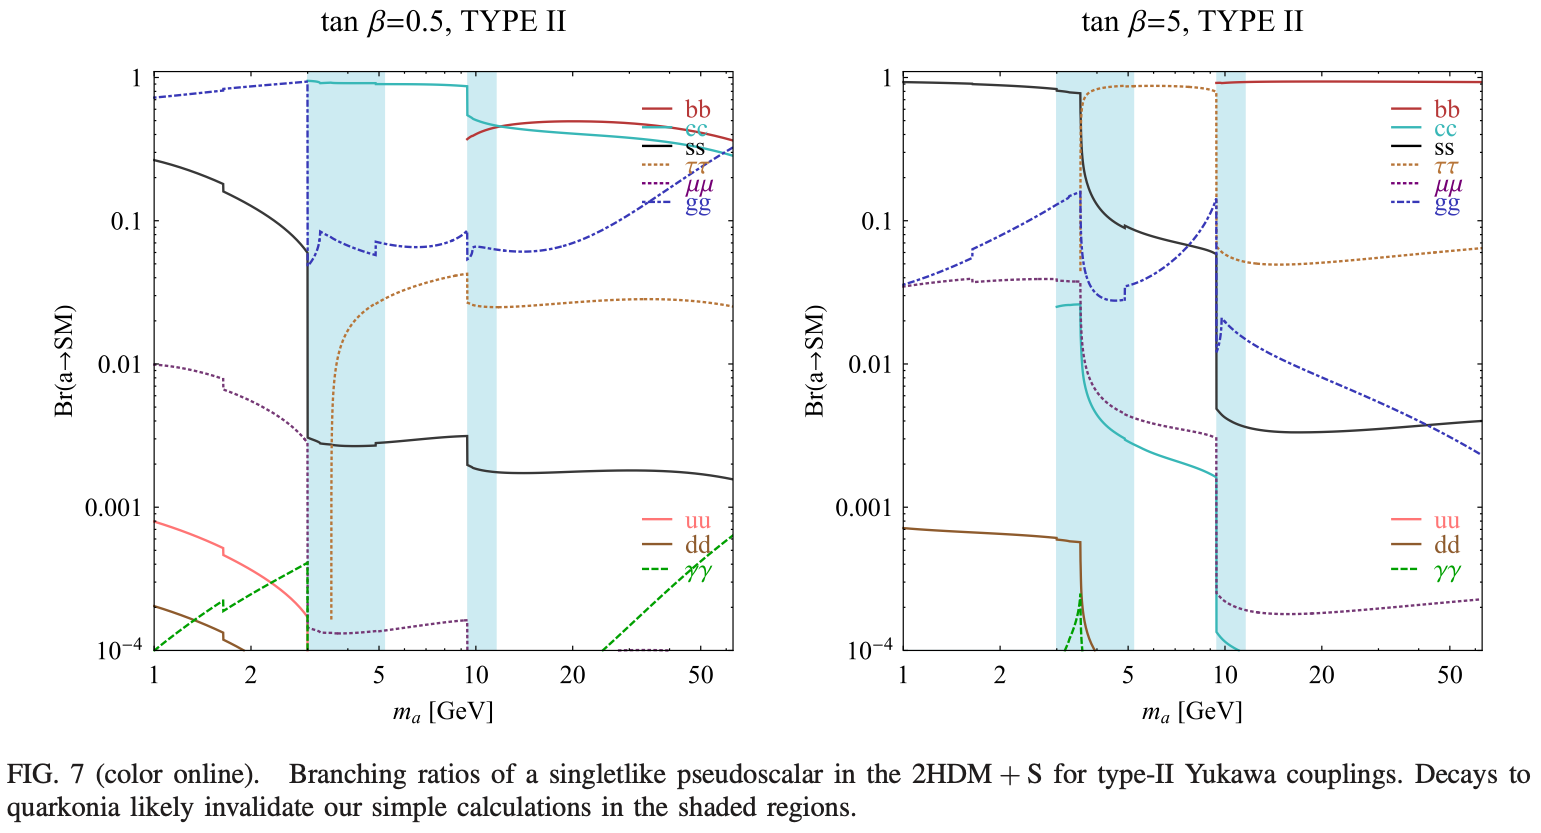
\includegraphics[width=15cm]{figures/curtin-2014-figure-7-BRs-of-singlelike-pseudoscalar-type-II.png}
    \caption{Figure 7 from Curtin et al. (2014): Branching ratios of a singlet-like pseudsocalar in Type II 2HDM+S for $tan\beta = 0.5$ (left) and $\tan\beta = 5$ (right), showing the dependence of the branching ratios on $\tan\beta$, as well as the prominence of the branching ratios to $bb$ and $\tau\tau$, the channels searched for in the analysis presented here.}
    \label{fig:curtin-2014-fig-4-typeI-BRs}
\end{figure}


% [CITE] continue citing https://journals.aps.org/prd/pdf/10.1103/PhysRevD.90.075004, before equation 14
In 2HDM, and by extension 2HDM+S, there are four types of fermion couplings commonly discussed in the literature that forbid flavour-changing neutral currents at tree level. These are referred to as Type I (all fermions couple to $H_2$), Type II (MSSM-like, $d_R$ and $e_R$ couple to $H_1$, $u_R$ to $H_2$), Type III (lepton-specific, leptons and quarks couple to $H_1$ and $H_2$ respectively) and Type IV (flipped, with $u_R$, $e_R$ coupling to $H_2$ and $d_R$ to $H_1$). The exact branching ratios of the pseudoscalars to Standard Model particles vary depending on the 2HDM+S model and the value of $\tan\beta$ (e.g. Fig. \ref{fig:curtin-2014-fig-4-typeI-BRs}).

\subsection{Two Real Singlet Model}
% [CITE] https://arxiv.org/pdf/1908.08554.pdf 
The two real singlet model (TRSM) adds two real singlet degrees of freedom to the Standard Model. These are written as two real singlet fields $S$ and $X$. Depending on the vacuum expectation values acquired by the scalars, different phases of the model can be realized. To reduce the number of free parameters, two discrete $\mathbb{Z}_2$ symmetries are introduced. The fields are decomposed as

\begin{equation}
    \Phi = \begin{pmatrix} 0 \\ \frac{\phi_h + v}{\sqrt{2}} \end{pmatrix}, 
    \,
    S = \frac{\phi_S + v_S}{\sqrt{2}} ,
    \,
    X = \frac{\phi_X + v_X}{\sqrt{2}}
\end{equation}
To achieve electroweak-breaking symmetry, $v  = v_{SM} \sim 246$ 246 GeV is necessary. If the vacuum expectation values $v_S, v_X \neq 0$ the $\mathbb{Z}_2$ are spontaneously broken, and the fields $\phi_{h,S,X}$ mix into three physical scalar states. This is called the broken phase and leads to the most interesting collider phenomenology.

The mass eigenstates $h_{1,2,3}$ are related to the fields $\phi_{h,S,X}$ through a $3\times 3$ orthogonal mixing matrix denoted $R$. The mass eigenstates are assumed to be ordered $M_1 \leq M_2 \leq M_3$. $R$ is parametrized by the three mixing angles $\theta_{hS}$, $\theta_{hX}$, $\theta_{SX}$. The nine parameters of the scalar potential can be expressed in terms of the three physical Higgs masses, the three mixing angles, and the three vacuum expectation values. 

After fixing one of the Higgs masses to the mass of the observed Higgs boson, and fixing the Higgs doublet vacuum expectation value to its Standard Model value, there are seven remaining free parameters of the TRSM.

In one benchmark scenario of TRSM, the heaviest scalar state $h_3$ is identified with the 125 GeV Higgs, $h_{125}$, and it can decay asymmetrically $h_{125} \rightarrow h_1 h_2$, which we also denote $h \rightarrow a_1 a_2$ to highlight the similarity with the symmetric decay $h \rightarrow aa$ typically interpreted in 2HDM+S as discussed. The parameter values in TRSM are chosen such that the coupling of $h_3$ to Standard Model particles are nearly identical to the Standard Model predictions. 

\begin{figure}[ht]
    \centering
    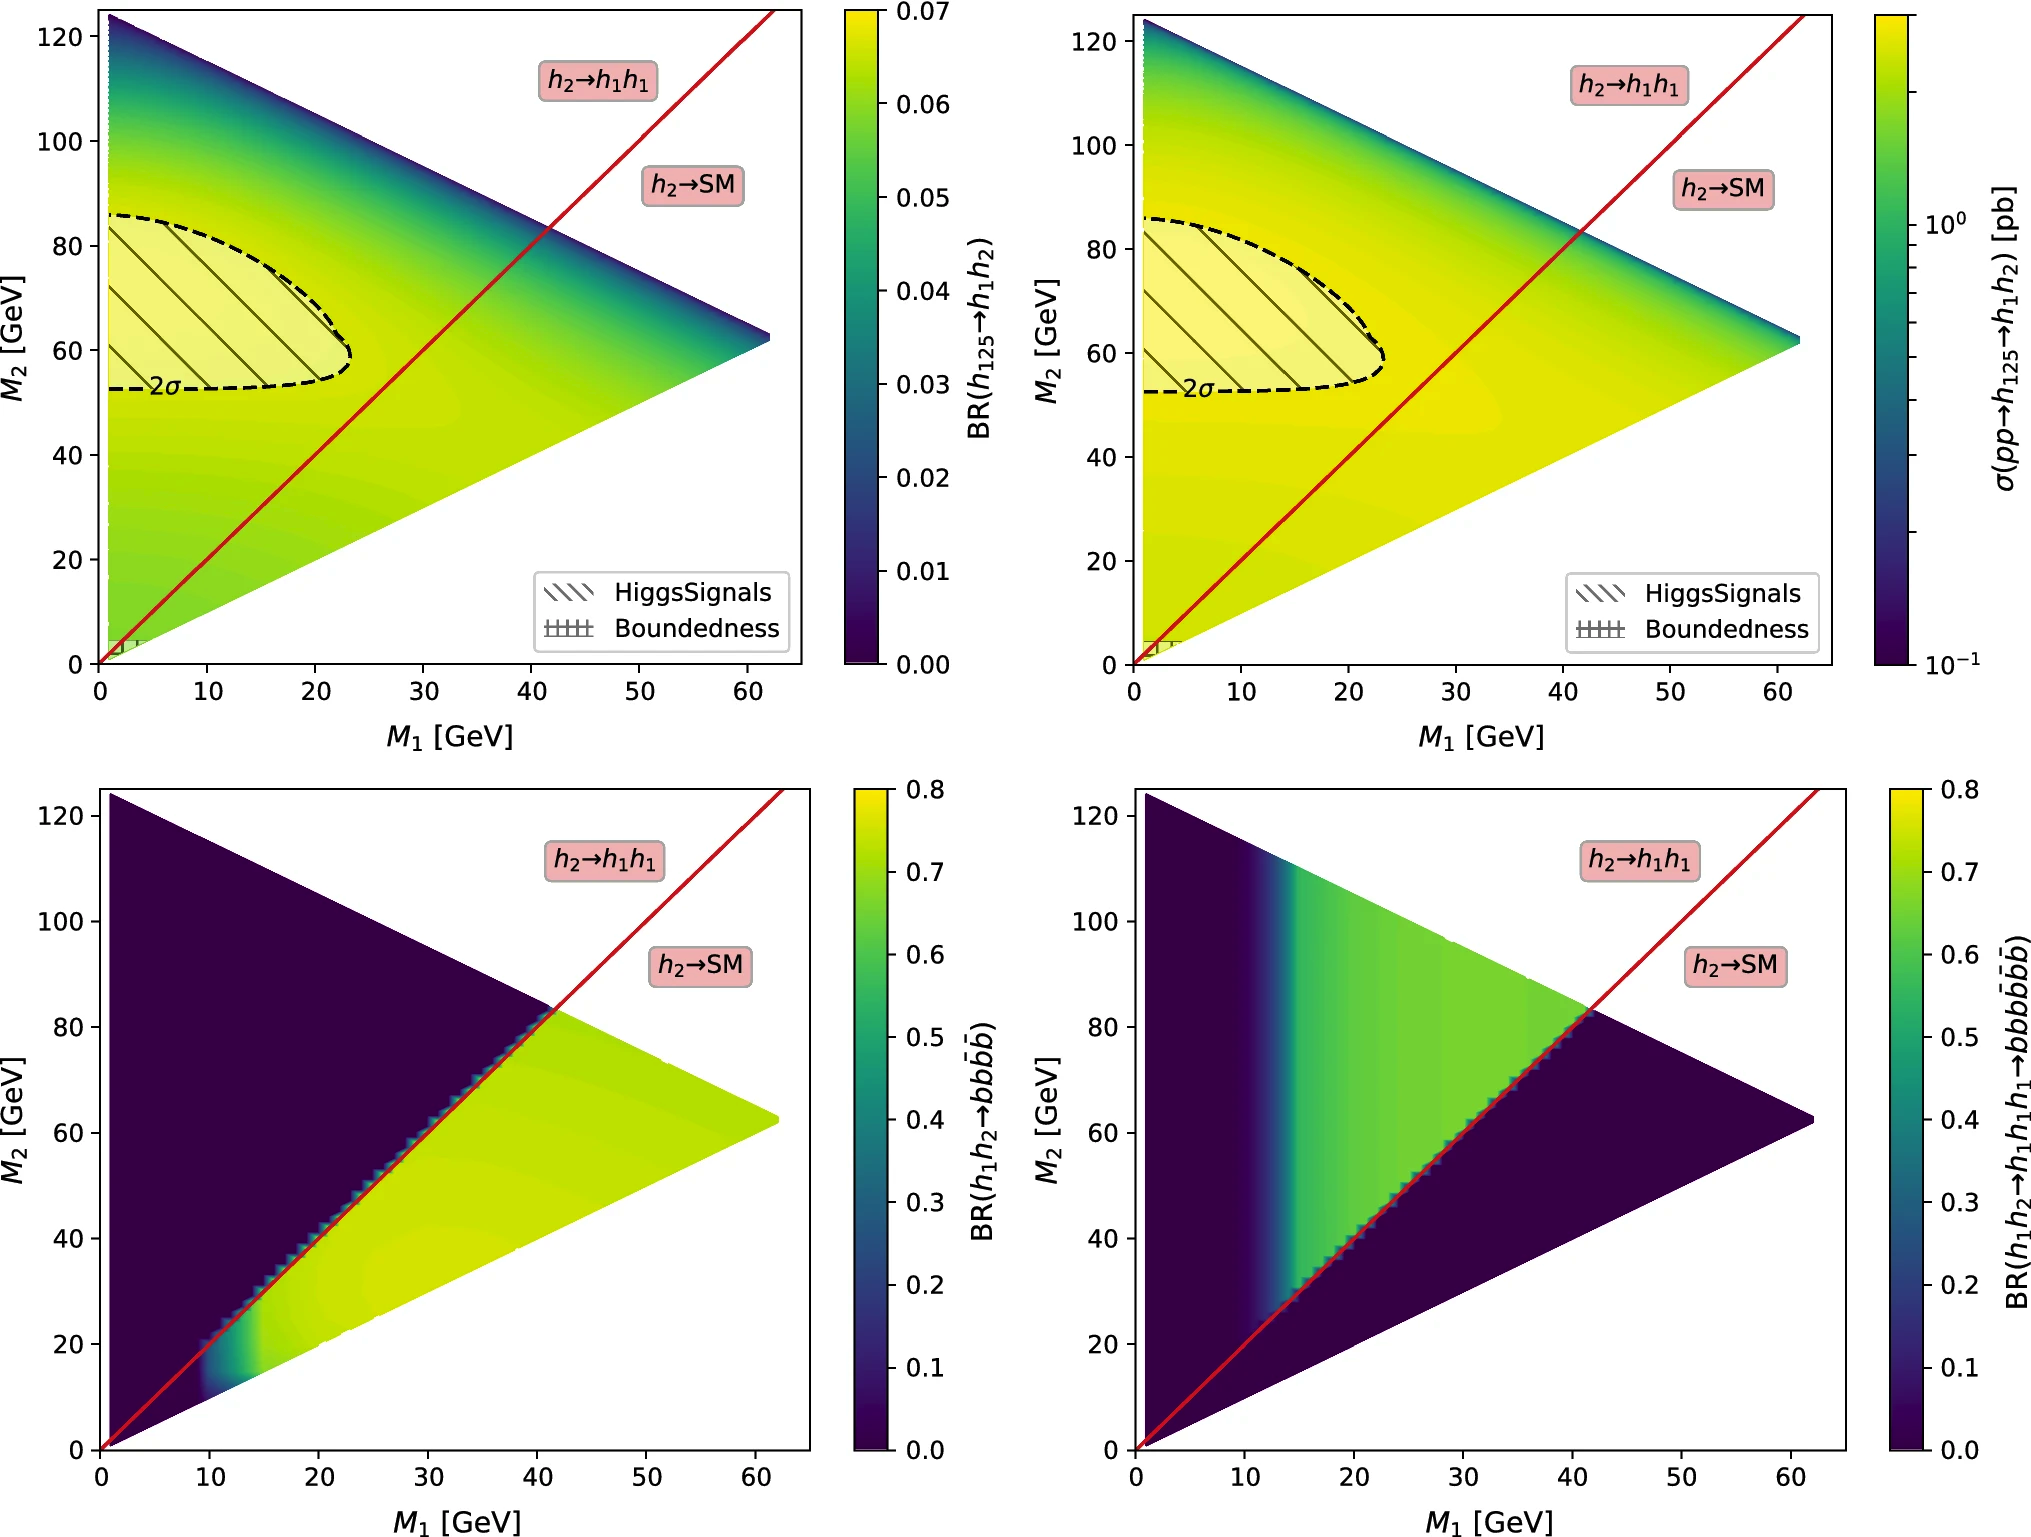
\includegraphics[width=15cm]{figures/Robens-TRSM-Figure-6-BP-1.png}
    \caption{Benchmark plane BP1 for benchmark scenario 1 from [CITE] Robens et. al, for the decay signature $h_{125} \rightarrow h_1 h_2$ with $h_{125} \equiv h_3$, defined in the $(M_1, M_2)$ plane. The color code shows BR$(h_3 \rightarrow h_1 h_2)$ (\textit{top left}) and the 13 TeV LHC signal rate for $pp \rightarrow h_3 \rightarrow h_1 h_2$ (\textit{top right}). The red line separates the region $M_2 > 2 M_1$, where BR($h_2 \rightarrow h_1 h_1$) $\sim 100\%$, from the region $M_2 < 2 M_1$, where BR($h_2 \rightarrow F_{SM}$) $\sim 100\%$. The \textit{bottom left} and \textit{right} show the branching ratio of the $h_1 h_2$ into (respectively) $b\bar{b}b\bar{b}$, and through a $h_2 \rightarrow h_1 h_1$ cascade to $b\bar{b}b\bar{b}b\bar{b}$. The hatched region indicates where the decay rate slightly exceeds the $2\sigma$ upper limit inferred from the LHC Higgs rate measurements, though the region depends on the parameter choices and experimental searches should cover the whole mass range.}
    \label{fig:trsm_bp1}
\end{figure}

In benchmark scenario 1 (benchmark plane 1, or BP1) (Fig. \ref{fig:trsm_bp1} from [CITE] Robens et. al), the maximal branching ratios for $h_3 \rightarrow h_1 h_2$ reach up to $7-8\%$ which translates into a signal rate of around 3 pb. These maximal branching ratios are reached in the intermediate mass state for $h_2$, $M_2 \sim 60 - 80$ GeV. For $M_2 < 40$ GeV, although phase space opens up significantly for light decay products, the branching ratio becomes smaller. 

If the decay channel $h_2 \rightarrow h_1 h_1$ is kinematically open (i.e. $M_2 > 2M_1$), it is the dominant decay mode leading to a significant rate for the $h_1 h_1 h_1$ final state, which we call a \textbf{cascade} decay. In BP1, $BR(h_2 \rightarrow h_1h_1$) $\simeq 100\%$ above the red line in Fig. \ref{fig:trsm_bp1}. If, in addition, $M_1 \gtrsim 10$ GeV, the $h_1$ decays dominantly to $b\bar{b}$ leading to a sizable rate for the $b\bar{b}b\bar{b}b\bar{b}$ final state as shown in Fig. \ref{fig:trsm_bp1} (\textit{bottom right}).

If the $h_2 \rightarrow h_1 h_1$ decay is kinematically closed (i.e. $M_2 < 2M_1$), both scalars decay directly to Standard Model particles, with branching ratios identical to a Standard Model-like Higgs boson, i.e. with the $b\bar{b}b\bar{b}$ final state dominating, as shown in Fig. \ref{fig:trsm_bp1} (\textit{bottom left}), while at smaller masses, combinations with $\tau$ leptons and eventually final states with charm quarks and muons become relevant.

\section{Sources}

    \begin{itemize}
        \item \texttt{https://www.space.com/standard-model-physics}
        \item \texttt{https://www.iop.org/explore-physics/big-ideas-physics/standard-model}
        \item Wikipedia
        \item \texttt{https://www.damtp.cam.ac.uk/user/tong/sm/standardmodel1.pdf}
    \end{itemize}

\end{document}